\subsection{Visão geral}
Este teste visou testar a aplicabilidade da base magnética comercial do
fabricante MagTek, modelo PME-300, no ambiente da turbina. A base magnética
comercial é projetada para aderir a superfícies planas ou cilíndricas convexas.
No caso da turbina, as regiões testadas têm formatos variados, que dependendo da
orientação da base, podem ser cilíndricos côncavos ou convexos. As
superfícies também variam de material, tratamento superficial e pintura,
assim como limpeza e rugosidade.

Por esse motivo viu-se a necessidade de testar
\textit{in situ} a base magnética comercial e verificar os reais limites de
adesão magnética do equipamento.


%---------------------------------------------------------------------
\subsection{Equipamentos utilizados}
\begin{enumerate}
  \item Base Magnética 300 kgf;
  \item Plataforma de apoio;
  \item Alavanca 0,8 m;
  \item Dinamômetro 25 kgf
\end{enumerate} 

\begin{figure}[h!]
\centering
	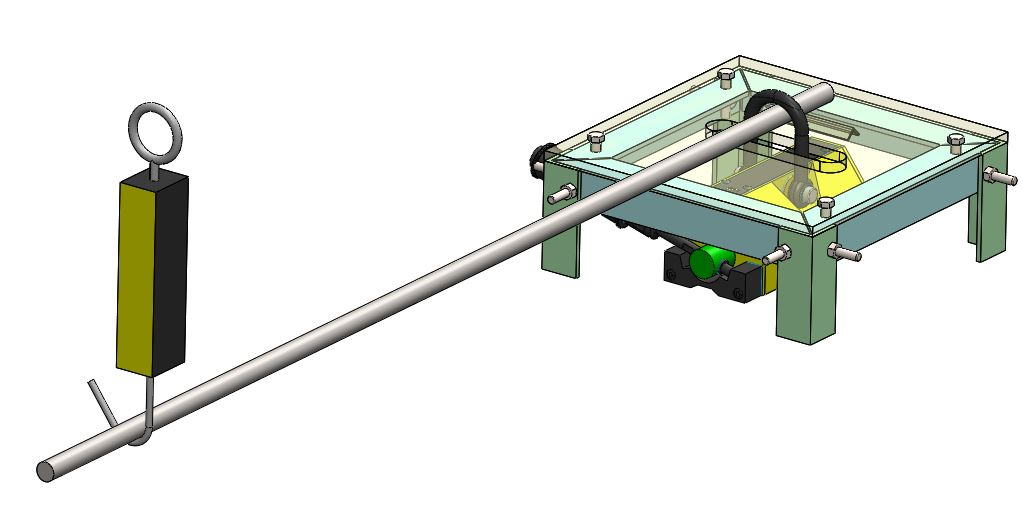
\includegraphics[width=0.9\columnwidth]{figs/conjunto_01.jpg}
	\caption{Conjunto de teste da base magnética}
	\label{fig::conjunto}
\end{figure}

\newpage
\subsection{Dados dos equipamentos}
\begin{description}
  \item[Base Magnética] \hfill
  \begin{itemize}
    \item Capacidade nominal: \\ [2ex]
	- no plano: 300 kgf \\
	- cilindro convexo: 150 kgf \\
	\item Capacidade máxima no plano: 960 kgf  
  \end{itemize}
  \item[Alavanca] \hfill \\
  De acordo com a figura~\ref{fig::esquematico}:
  \begin{itemize}
    \item Comprimento da alavanca: L
    \item Distância entre os apoios: d  	
  \end{itemize}
  Os valores de L e d foram medidos em cada resultado do teste e a razão
  L/d está indicada na tabela~\ref{table:1} da seção~\ref{sec::resultados}.
  \item[Dinamômetro] \hfill \\
  Capacidade máxima do dinamômetro: 25 kgf
\end{description}

\begin{figure}[h]
\centering
	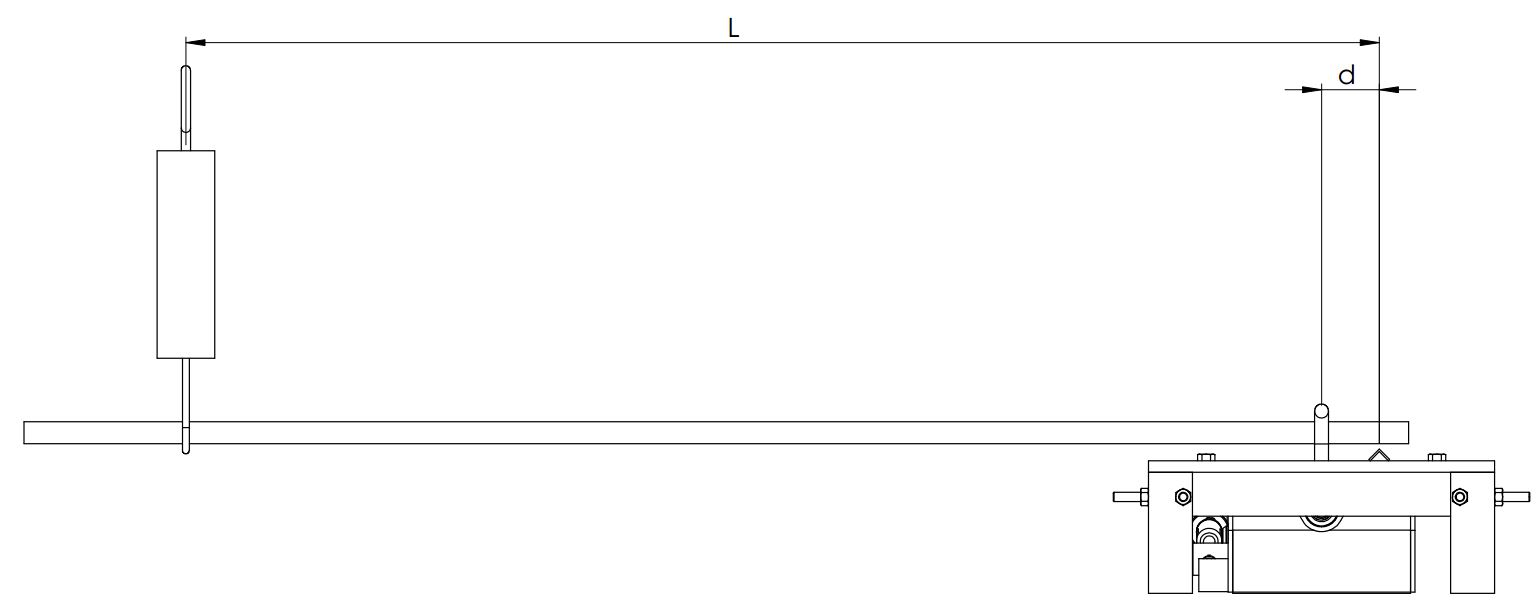
\includegraphics[width=0.9\columnwidth]{figs/esquematico.jpg}
	\caption{Esquemático da estrutura de teste com parâmetros de cálculo
	indicados}
	\label{fig::esquematico}
\end{figure}

%---------------------------------------------------------------------

\subsection{Cálculo da força magnética máxima}
A força magnética, em função da força medida no dinamômetro, está de acordo com
a equação~\ref{eq::fmag}:

\begin{equation} \label{eq::fmag}
F_{\text{mag}}=\frac{L}{d} F_{\text{din}}
\end{equation}


\subsection{Mapa de posicionamento} \label{sec::mapa}
Abaixo, apresenta-se um mapa esquemático das posições onde foram testadas a
adesão magnética da base.

\begin{figure}[h!]
\centering
	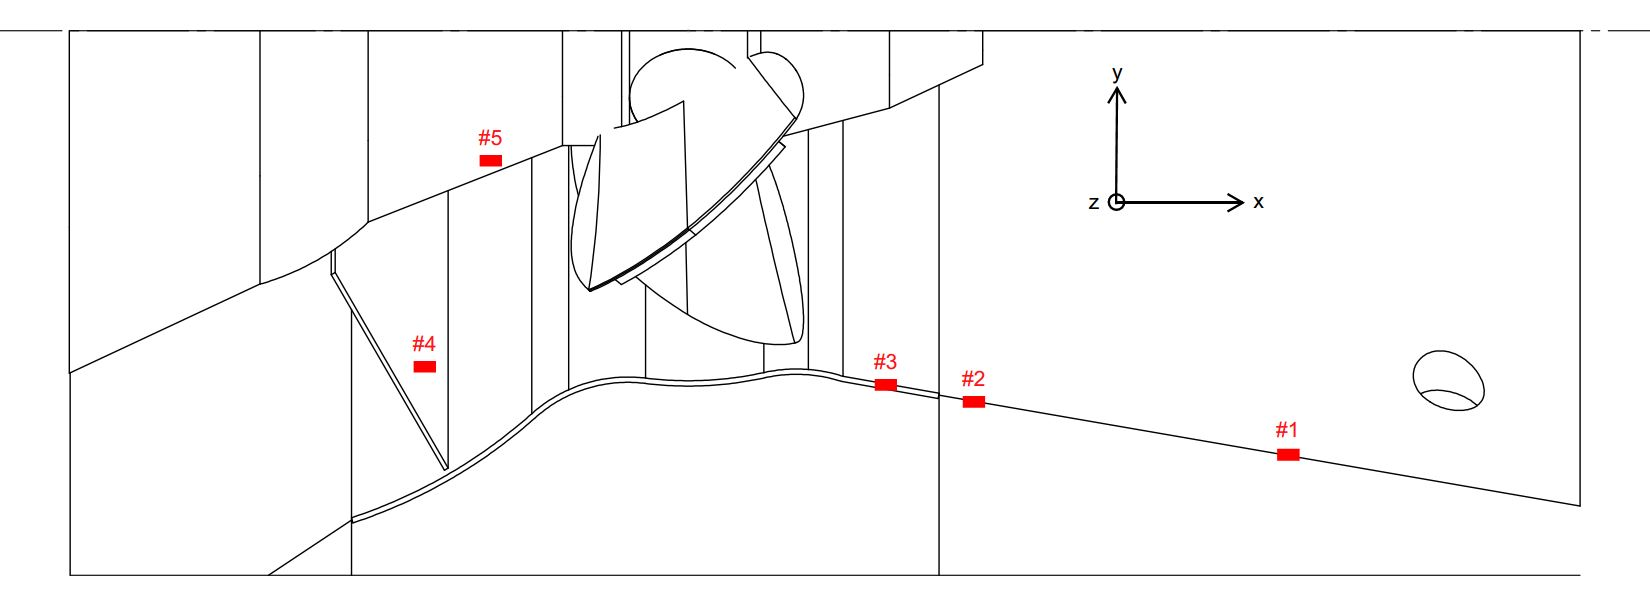
\includegraphics[width=0.8\columnwidth]{figs/mapa.jpg}
	\caption{Mapa esquemático de posições}
	\label{fig::mapa}
\end{figure}

\subsection{Procedimento} \label{sec::procedimento}
A adesão magnética foi testada nas posições indicadas no mapa esquemático da
seção~\ref{sec::mapa}. Para as posições 1 e 2 variou-se a orientação da base de
acordo com o eixo de coordenadas indicado na figura~\ref{fig::mapa}.

O procedimento de teste é o seguinte: 1) posiciona-se a base magnética; 2)
ativa-se o imã; 3) posiciona-se o apoio e a alavanca; 4) mede-se a distância
entre os apoios e o comprimento do braço de alavanca até o dinamômetro
(dimensões ''d'' e ''L''); 5) aplica-se gradualmente a carga na alavanca,
observando a indicação no dinamômetro, até que ocorra o primeiro dos dois casos:
a) o dinamômetro indica a carga máxima, ou b) a base magnética descola-se da
superfície; 6) anota-se o resultado.

\begin{figure}[h!]
\centering
	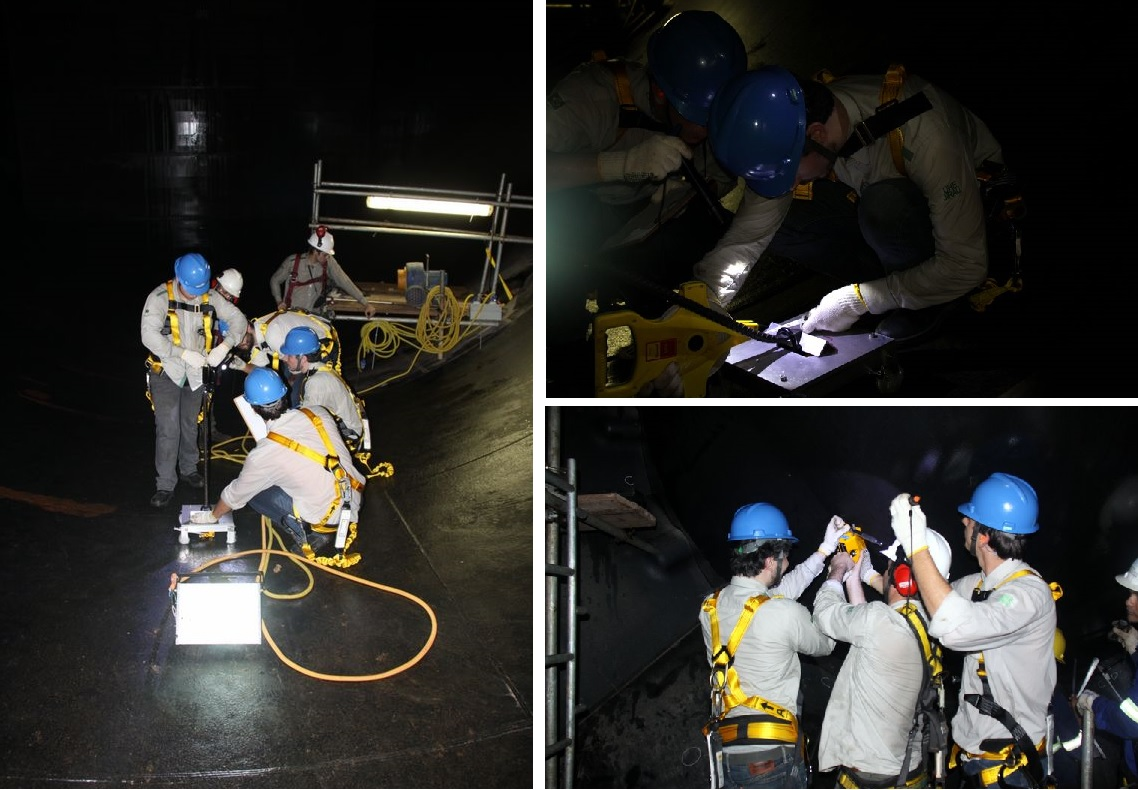
\includegraphics[width=0.5\columnwidth]{figs/fotos.jpg}
	\caption{Fotos durante o teste}
	\label{fig::fotos}
\end{figure}

\subsection{Resultados} \label{sec::resultados}
A tabela~\ref{table:1} apresenta o resultado do teste da base magnética nas
posições indicadas na seção~\ref{sec::mapa}.

\begin{table}[h!]
\centering
\begin{tabular}{||c c m{7em} m{4em} m{6em}||} 
 \hline
 Posição & Orientação & Força limite no dinamômetro (kgf) & L/d & Força
 magnética limite (kgf) \\  [0.5ex] 
 \hline\hline
 1 & x & 25 & 10,3 & 256 \\ 
 1 & x & 25 & 14,7 & 367 \\
 1 & x & 14 & 17,8 & 249 \\
 1 & z & 18 & 17,8 & 320 \\
 1 & x & 14 & 21,1 & 295 \\
 2 & z & 12 & 22,9 & 274 \\
 2 & x & 8,5 & 21,1 & 179 \\
 2 & xz 45º & 10 & 22,9 & 229 \\
 3 & x & 0 & 22,9 & 0 \\
 3 & z & 0 & 22,9 & 0 \\
 4 & n/a & n/a & n/a & n/a \\
 5 & n/a & n/a & n/a & n/a \\ [1ex]
 \hline
\end{tabular}
\caption{Resultados do teste experimental}
\label{table:1}
\end{table}

%---------------------------------------------------------------------

\subsection{Conclusões}
O teste possibilitou verificar a capacidade de adesão magnética para diferentes
posições, geometria de superfície e materiais no interior da turbina. O maior
valor encontrado, de 367 kgf, é superior até à capacidade de carga nominal para
superfícies planas indicada pelo fabricante. O menor valor encontrado, de 179
kgf ainda é superior ao valor máximo para superfícies cilíndricas, indicado pelo
fabricante.

Desta forma, considera-se que os valores nominais do equipamento fornecem uma
boa referência para o dimensionamento deste equipamento como base para uma
amarração robusta da solução mecânica do projeto.

A posição 3, de acordo com o mapa esquemático da seção~\ref{sec::mapa}, é uma
região composta por aço inoxidável e não forneceu adesão magnética. As posições
4 e 5 são respectivamente a superfície das paletas do distribuidor e a
superfície do rotor. Estas superfícies apresentaram boa adesão magnética, mas
não foi possível medir valores limite, pois tais posições não estavam previstas
no teste e o equipamento projetado não permitiria uma medição adequada.